\section{Ceph RADOS}

\begin{frame}{Cluster Aware}
    Where should the object be placed
    \begin{itemize}
        \item \textbf{Traditional}
            \begin{itemize}
                \item Centralized interface provides services to the client through a double dispatch
                \item Huge bottleneck at petabyte-to-exabyte scale.
            \end{itemize}
        \item \textbf{Ceph}
            \begin{itemize}
                \item Ceph OSD and Client are \textit{cluster aware}
                \item Each OSD knows about other OSD in the cluster
                \item OSD can interact directly with other OSD and monitors
                \item Client can interact directly with OSD
            \end{itemize}
    \end{itemize}
\end{frame}

%\begin{frame}{Cluster Aware}
%    \begin{itemize}
%        \item \textbf{OSDs Service Clients Directly}
%        \item \textbf{OSD Membership and Status}
%        \item \textbf{Data Scrubbing}
%        \item \textbf{Replication}
%    \end{itemize}
%\end{frame}

\begin{frame}{Cluster Map}
    Cluster Map indicates the knowledge of the cluster topology.
    \begin{itemize}
        \item \textbf{The Monitor Map}
        \item \textbf{The OSD Map}
        \item \textbf{The PG Map}
        \item \textbf{The CRUSH Map}
        \item \textbf{The MDS Map} 
    \end{itemize}
\end{frame}

\begin{frame}[fragile]{Cluster Map: Monoitor Map}
\begin{lstlisting}[language=python]
ubuntu@ip-172-31-58-195:~# ceph mon dump
dumped monmap epoch 2
epoch 2
fsid ccb00027-ca55-48cc-bf5a-b6cbf79c9b99
last_changed 2018-12-26 18:17:17.540294
created 2018-12-26 18:16:44.542161
0: 172.31.56.105:6789/0 mon.ip-172-31-56-105
1: 172.31.57.232:6789/0 mon.ip-172-31-57-232
2: 172.31.58.195:6789/0 mon.ip-172-31-58-195 
\end{lstlisting}
\end{frame}

\begin{frame}[fragile]{Cluster Map: OSD Map}
\begin{lstlisting}[language=python]
ubuntu@ip-172-31-58-195:~# ceph osd dump
epoch 245
fsid ccb00027-ca55-48cc-bf5a-b6cbf79c9b99
created 2018-12-26 18:17:10.141095
modified 2018-12-29 12:02:43.764006
crush_version 26
...
pool 5 'cephfs_data' replicated size 3 min_size 2 crush_rule 0 object_hash rjenkins pg_num 64 pgp_num 64 last_change 48 flags hashpspool stripe_width 0 application cephfs
pool 6 'cephfs_metadata' replicated size 3 min_size 2 crush_rule 0 object_hash rjenkins pg_num 64 pgp_num 64 last_change 48 flags hashpspool stripe_width 0 application cephfs
max_osd 4
osd.0 up   in  weight 1 up_from 98 up_thru 244 down_at 94 last_clean_interval [90,93) 172.31.56.105:6801/2052 172.31.56.105:6802/2052 172.31.56.105:6803/2052 172.31.56.105:6804/2052 exists,up 2ee23b61-eca4-41e5-a6b0-277bfd6c48a1
...
\end{lstlisting}
\end{frame}

\begin{frame}[fragile]{Cluster Map: CRUSH Map}
\begin{lstlisting}[language=python]
ubuntu@ip-172-31-58-195:~# ceph osd tree
ID CLASS WEIGHT  TYPE NAME                 STATUS REWEIGHT PRI-AFF
-1       0.11597 root default
-3       0.02899     host ip-172-31-56-105
 0   ssd 0.02899         osd.0                 up  1.00000 1.00000
-5       0.02899     host ip-172-31-57-232
 1   ssd 0.02899         osd.1                 up  1.00000 1.00000
-7       0.02899     host ip-172-31-58-195
 2   ssd 0.02899         osd.2                 up  1.00000 1.00000
-9       0.02899     host ip-172-31-61-170
 3   ssd 0.02899         osd.3               down        0 1.00000
\end{lstlisting}
\end{frame}

\begin{frame}{Cluster Map}
    \begin{itemize}
        \item 由若干个monitor共同负责整个Ceph集群中所有的OSD状态的发现与记录,并且共同形成cluster map的master版本,然后扩散到整体OSD以及client
        \item OSD使用cluster map进行数据的维护,client使用cluster进行数据的寻址
        \item monitor并不主动轮询各个OSD的当前状态。正相反,OSD需要向monitor上报状态信息。常见的上报有两种情况
            \begin{itemize}
                \item 新的OSD被加入集群
                \item 某个OSD发现自身或者其他OSD发生异常
            \end{itemize}
        \item 在收到这些上报信息后,monitor将更新cluster map信息并加以扩散
    \end{itemize}
\end{frame}

\begin{frame}{Data Operation Procedure}
    \begin{figure}[htpb]
        \centering
        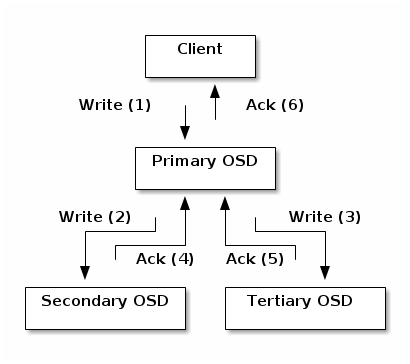
\includegraphics[width=0.6\linewidth]{file-write.png}
    \end{figure}
\end{frame}

\subsection{Map Changes and Data Movement}

\begin{frame}{Peering and Recovery}
    The Ceph Object Store is dynamic
    \begin{itemize}
        \item \textbf{Failure is the norm rather than the exception}
        \item \textbf{The cluster map records cluster state at a point in time}
        \item \textbf{The cluster map contains the OSDs status(up/down, weight, IP)}
            \begin{itemize}
                \item OSDs cooperatively migrate data
                \item They do so to achieve recovery based on CRUSH rules
                \item Any cluster map update potentially triggers data migration
            \end{itemize}
    \end{itemize}
\end{frame}

%\begin{frame}{Failure is the norm}
%    \begin{itemize}
%        \item \textbf{ceph-osd daemon dies}
%            \begin{itemize}
%                \item Peer heartbeats fail; peers inform monitor
%                \item New osdmap published with osd.123 as \textit{down}
%            \end{itemize}
%        \item \textbf{pg maps to fewer replicas}
%            \begin{itemize}
%                \item If osd.123 was primary in a PG, a replica takes over
%                \item PG is \textit{degraded}(N-1 replicas)
%                \item Data redistribution is not triggered
%            \end{itemize}
%        \item \textbf{Monitor marks OSD \textit{out} after 5 minutes}
%            \begin{itemize}
%                \item PG now maps to N OSDs again
%                \item PG re-peers, activates
%                \item Primary backfills to the \textit{new} OSD 
%            \end{itemize}
%    \end{itemize}
%\end{frame}

\begin{frame}{CRUSH}
    \begin{figure}[htpb]
        \centering
        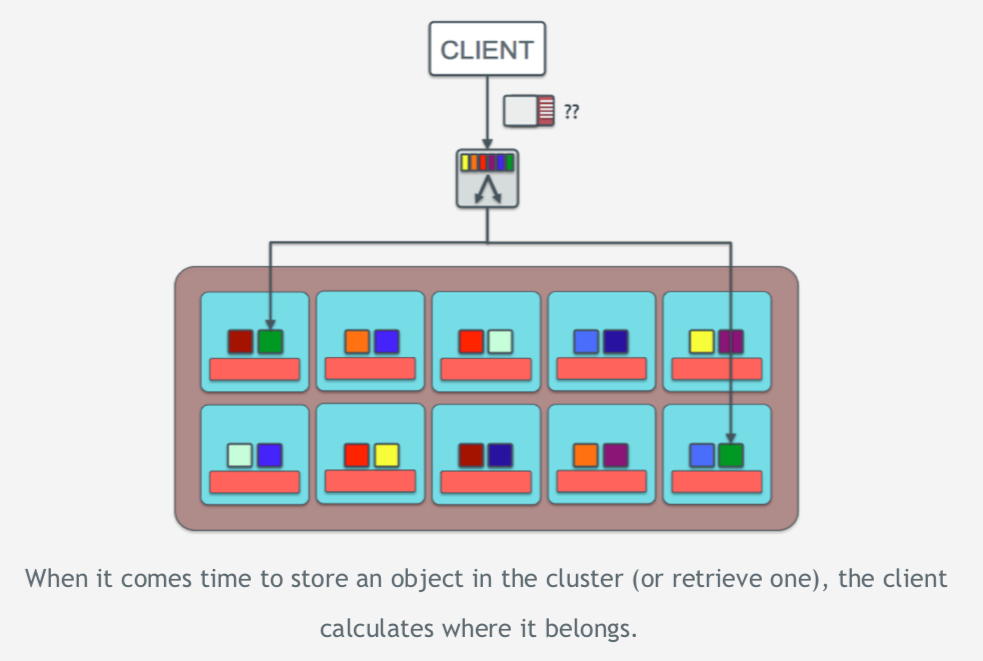
\includegraphics[width=0.8\linewidth]{migration1.png}
    \end{figure}
\end{frame}

\begin{frame}{CRUSH}
    \begin{figure}[htpb]
        \centering
        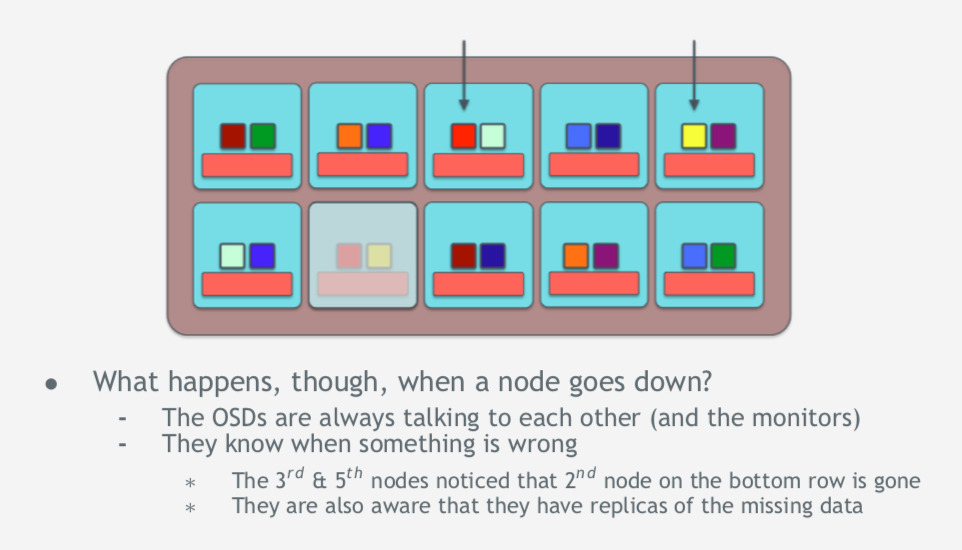
\includegraphics[width=0.8\linewidth]{migration2.png}
    \end{figure}
\end{frame}

\begin{frame}{CRUSH}
    \begin{figure}[htpb]
        \centering
        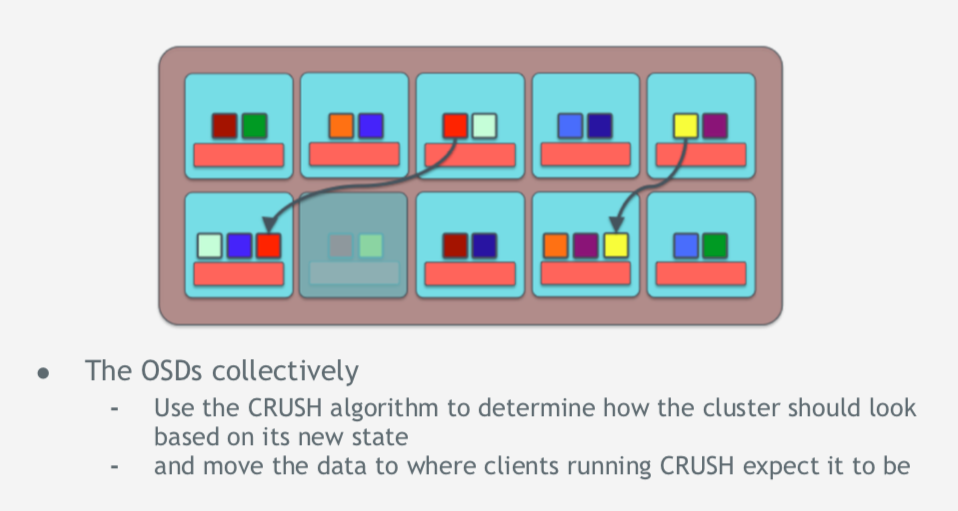
\includegraphics[width=0.8\linewidth]{migration3.png}
    \end{figure}
\end{frame}

\begin{frame}{CRUSH}
    \begin{figure}[htpb]
        \centering
        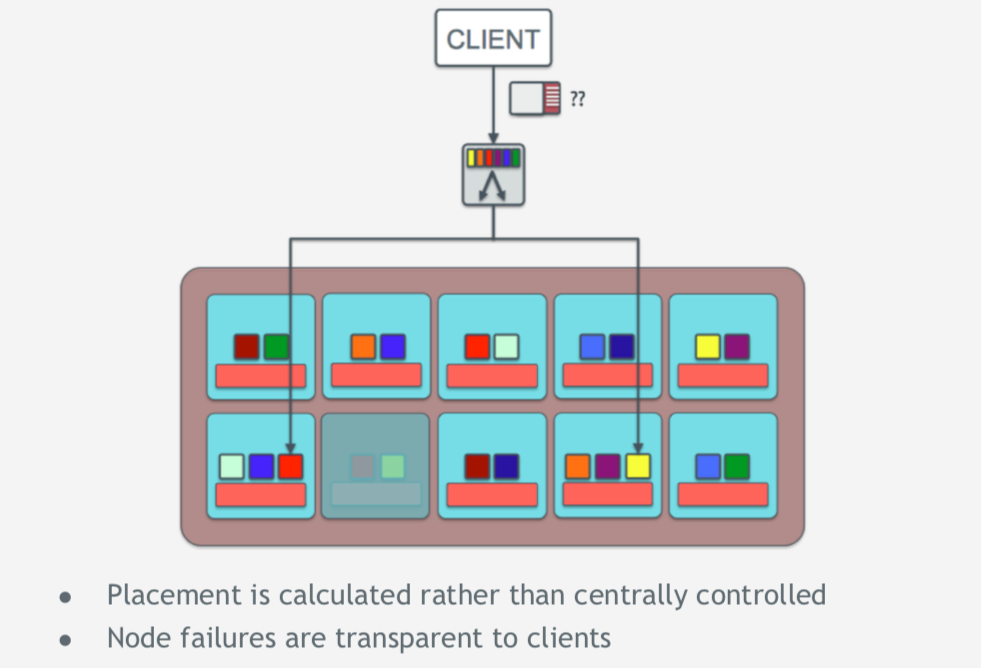
\includegraphics[width=0.8\linewidth]{migration4.png}
    \end{figure}
\end{frame}

\begin{frame}{OSD Fail}
    \begin{figure}[htpb]
        \centering
        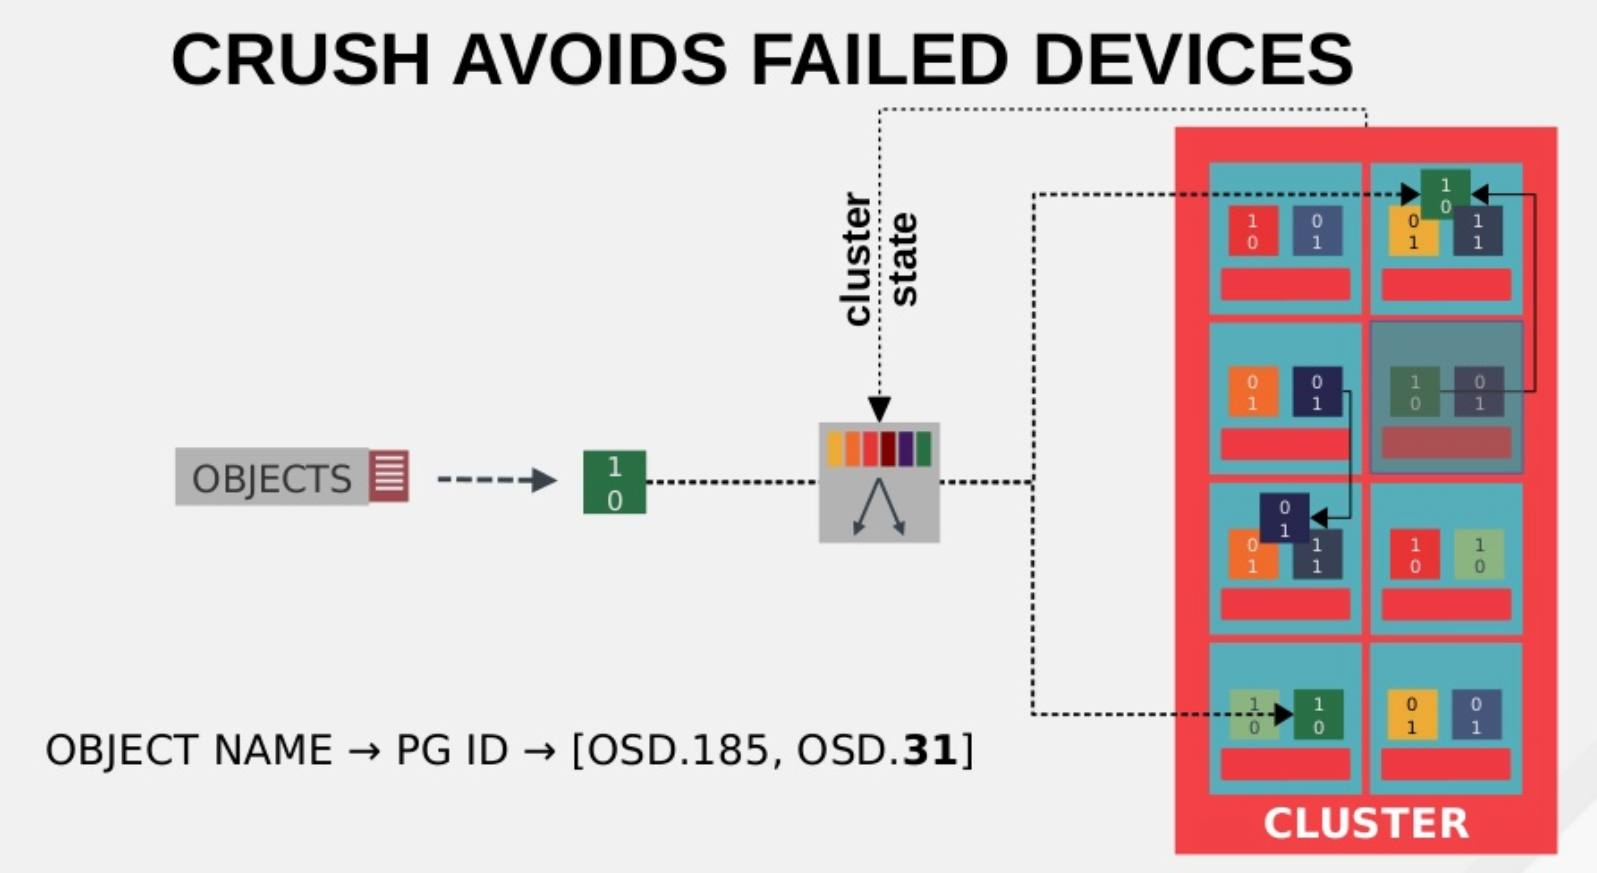
\includegraphics[width=1\linewidth]{crush-failed-device.png}
    \end{figure}
\end{frame}

%\begin{frame}{OSD Expansion}
%    \begin{itemize}
%        \item New rack of OSDs added to CRUSH map
%        \item Many PGs map to new OSDs
%            \begin{itemize}
%                \item Temporarily remap PG to include previous replicas + new OSDs keeps replica count at (or above) target
%                \item Peer and activate
%                \item Background backfill to new OSDs
%                \item Drop re-mapping when completed, activate
%                \item Delete PG data from the old \textit{stray} replica 
%            \end{itemize}
%    \end{itemize}
%\end{frame}
%

\begin{frame}[fragile]{Python S3 Example}
\begin{lstlisting}[language=python]
# creating a connection
conn = boto.connect_s3(aws_access_key_id = access_key,
    aws_secret_access_key = secret_key,
    host = 'objects.dreamhost.com',
    calling_format = boto.s3.connection.OrdinaryCallingFormat())

# listing owned buckets
for bucket in conn.get_all_buckets():
    print "{name}\t{created}".format(name = bucket.name, created = bucket.creation_date)
# mahbuckat1   2011-04-21T18:05:39.000Z
# mahbuckat2   2011-04-21T18:05:48.000Z

# listing a bucket's content
for key in bucket.list():
    print "{name}\t{size}\t{modified}".format(name = key.name, size = key.size, modified = key.last_modified)
# myphoto1.jpg 251262  2011-08-08T21:35:48.000Z
# myphoto2.jpg 262518  2011-08-08T21:38:01.000Z

# creating an object
key = bucket.new_key('hello.txt')
key.set_contents_from_string('Hello World!')

# download an object to a file
key = bucket.get_key('perl_poetry.pdf')
key.get_contents_to_filename('/home/larry/documents/perl_poetry.pdf')

\end{lstlisting}
\end{frame}
